\section{Virtualization}
\sectionslide{Virtualization}
\begin{frame}
	\frametitle{Virtualization}
	\begin{columns}
		\column{.5\textwidth}		
		
		Classical view of \textbf{a computer} running \textbf{an operating system}, running \textbf{a program}.
		\vspace{0.5cm}
		\begin{itemize}
			\item OS is in full control of the hardware
			\item A program runs with lower privilege
			\item OS assigns resources to program
		\end{itemize}
		\vspace{0.5cm}
		OS acts as a \textbf{supervisor} for programs.
		
		\column{.5\textwidth}
		\centering
		\begin{tikzpicture}
			\node[] (comp) at (0,0) {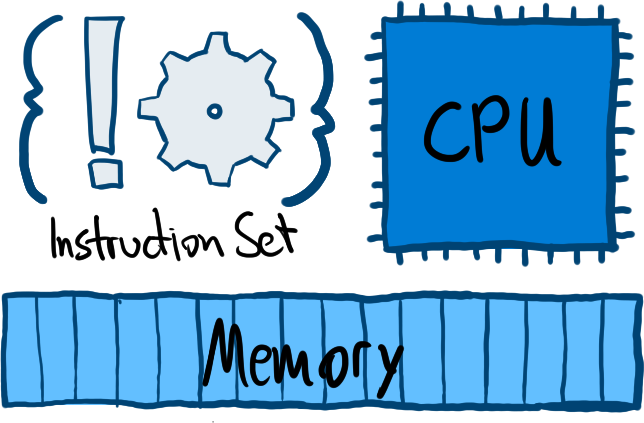
\includegraphics[width=5.6cm]{pics/computer.png}};
			\node[] (os) [above=0cm of comp] {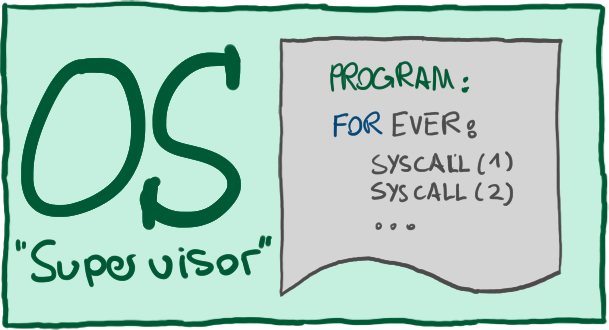
\includegraphics[width=5.6cm]{pics/os_prog.png}};
		\end{tikzpicture}
		
	\end{columns}	
\end{frame}

\begin{frame}
	\frametitle{Virtualization}
	\begin{columns}
		\column{.6\textwidth}
		\begin{block}{Virtual Machine Monitor\footnotemark[1] (\textbf{Hypervisor})}
			\begin{enumerate}
				\item provides environment essentially identical to original machine
				\item in full control of system resources
				\item Programs run with minimal speed decreases in this environment
			\end{enumerate}
		\end{block}
	
		\begin{block}{Virtual Machine\footnotemark[1]}
			The environment for \textbf{programs} to run in, with a \textbf{Hypervisor} present, is called a \textbf{Virtual Machine}.
		\end{block}
		
		\column{.4\textwidth}
		\centering
		\begin{tikzpicture}
			\node[] (comp) at (0,0) {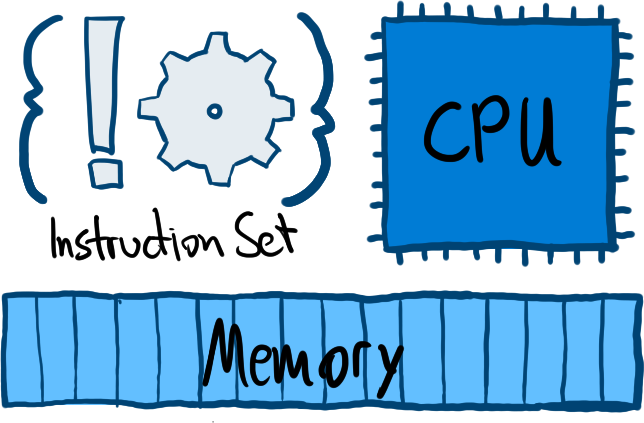
\includegraphics[width=4.6cm]{pics/computer.png}};
			\node[] (hyp) [above=-0.2cm of comp] {
\includegraphics[width=4.6cm]{pics/hypervisor.png}};
			\node[] (os) [above=-0.2cm of hyp] {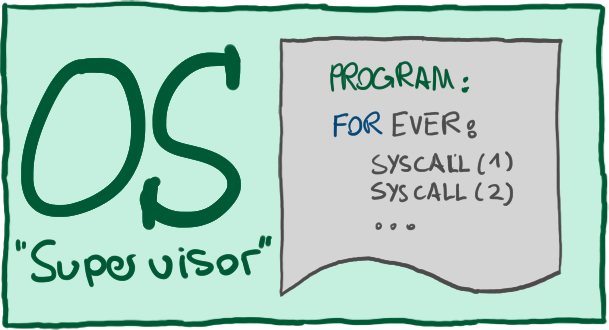
\includegraphics[width=4.6cm]{pics/os_prog.png}};
		\end{tikzpicture}
	\end{columns}
	\footnotetext[1]{\tiny Popek G.J., Goldberg R. P. \textit{Formal Requirements for Virtualizable Third Generation Architectures}, Commmunications of the ACM, Volume 7 (17), 1974}
	
\end{frame}

\section{Containers}
\sectionslide{Containers}
\begin{frame}
	\frametitle{"Containerization" - A kind of virtualization...}
	
	\begin{columns}
		\column{.55\textwidth}
			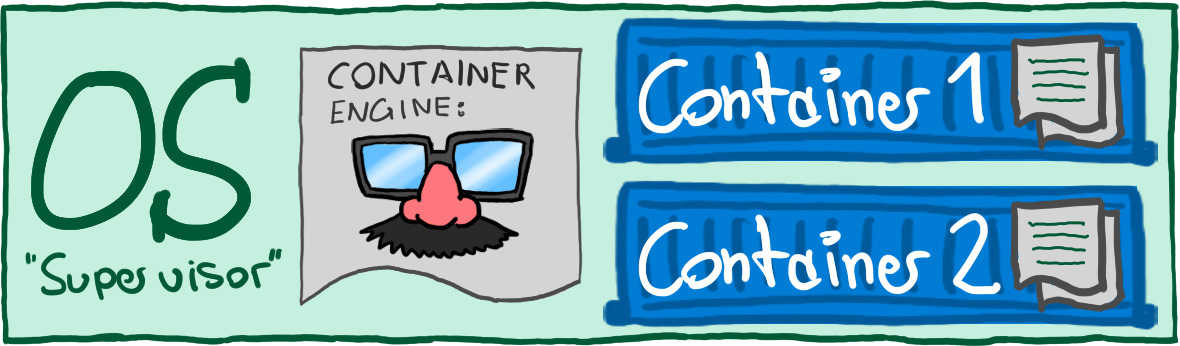
\includegraphics[width=.95\textwidth]{pics/os_cont.png}
			
		\column{.45\textwidth}
			\begin{block}{OS-level virtualization\footnotemark[1]}
				OS allows multiple instances of isolated user spaces (\textbf{containers}) to run applications in. They all share the OS Kernel.
			\end{block}
	\end{columns}

	\begin{columns}
		\column{.3\textwidth}
			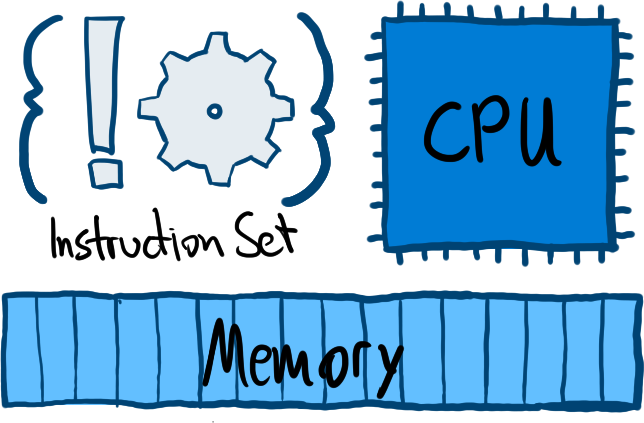
\includegraphics[width=\textwidth]{pics/computer.png}
		\column{.7\textwidth}
			\begin{itemize}
				\item Processes inside the container cannot see anything outside (processes, files, ...). Physically, they are processes running on the same OS Kernel, however.
				\item There is no need for a virtualization layer below the Kernel to run containers, although there can be one!
				\item A \hervor{container engine} or \hervor{runtime} manages the containers
			\end{itemize}
	\end{columns}
	
	\footnotetext[1]{\tiny\textit{OS-level Virtualization}, Wikipedia 2021, \href{https://en.wikipedia.org/wiki/OS-level\_virtualization}{https://en.wikipedia.org/wiki/OS-level\_virtualization}}
\end{frame}

\begin{frame}
	\frametitle{Containers}
	\begin{columns}
		\column{.45\textwidth}
		\begin{tikzpicture}
			\node[] (container) at (0,0) {
\includegraphics[width=.9\textwidth]{pics/container_large.png}};
			\node[] (image) [below=1cm of container] {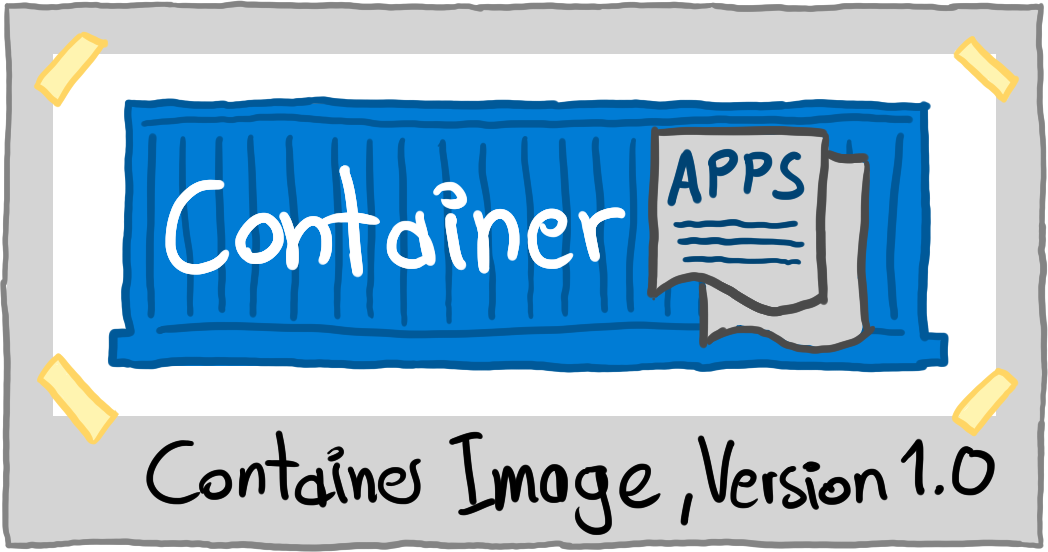
\includegraphics[width=.9\textwidth]{pics/container_image.png}};
			\draw[->, draw=mycolor, line width=5pt] (container)--(image);
		\end{tikzpicture}
		\column{.55\textwidth}
			\textbf{\Large Why?}
			\begin{itemize}
				\item Bundle up an application \hervor{with all its dependencies!}
				\item More \hervor{lightweight and portable} than a virtual machine
			\end{itemize}
		
			\vspace{.25cm}\textbf{\Large How?}
			\begin{itemize}
				\item Containers can be shipped as images (distribution infrastructure depends on system / engine)
				\item Who runs a container based on my image can be sure to have a \hervor{functionally identical environment}, independent of application type
			\end{itemize}
			
	\end{columns}
\end{frame}

\begin{frame}
	\frametitle{How to make containers?}
	\centering
	\textbf{Advanced use of Linux features!}
	\vspace{.5cm}\begin{columns}
		\column{.5\textwidth}
			\hervor{\Large namespaces}
			\begin{itemize}
				\item Limit what a process can \hervor{see}
				\item Change filesystem root with \codi{chroot}
				\item Change apparent \codi{pid}s
				\item ...
			\end{itemize}
		\column{.5\textwidth}
			\hervor{\Large cgroups}
			\begin{itemize}
				\item Limit what a process can \hervor{use}
				\item Hierarchical definition tree to assign quantities of memory, cpu cores, ... to processes and groups of processes
			\end{itemize}
	\end{columns}
	
	\centering
	\vspace{.5cm}Definitely watch those talks:
	\small
	\begin{itemize}
		\item Containers from scratch (Liz Rice, 2018): \myhref{https://www.youtube.com/watch?v=8fi7uSYlOdc}{https://www.youtube.com/watch?v=8fi7uSYlOdc}
		\item Namespaces, cgroups and beyond: What are containers made from? (Jérôme Petazzoni, 2015): \myhref{https://www.youtube.com/watch?v=sK5i-N34im8}{https://www.youtube.com/watch?v=sK5i-N34im8}
	\end{itemize}
	
	
\end{frame}

\begin{frame}
	\frametitle{Container runtimes / engines}
	
	\centering
	There are / might be several software layers between the user interacting with a \textbf{container engine} and the \textbf{runtime} that actually runs containers.
	
	\vspace{.3cm}\begin{columns}[t]
		\column{0.5\textwidth}
		Based on Linux namespaces and cgroups:
		\begin{itemize}
			\item \myhref{https://linuxcontainers.org/}{LXC}
			\item \myhref{https://www.docker.com/}{Docker} (Docker engine, containerd)
			\item \myhref{https://podman.io/}{Podman}
		\end{itemize}
	
		\column{.5\textwidth}
		Other mechanisms / systems:
		\begin{itemize}
			\item \myhref{https://docs.freebsd.org/en/books/arch-handbook/jail/}{FreeBSD Jail} (Unix)
			\item \myhref{https://docs.oracle.com/cd/E36784\_01/html/E36848/zones.intro-1.html\#scrolltoc}{Solaris Zones} (Unix)
			\item \myhref{https://docs.microsoft.com/en-us/virtualization/windowscontainers/quick-start/set-up-environment?tabs=Windows-Server}{Windows Containers}
		\end{itemize}
	\end{columns}

	
\end{frame}


